%\documentclass[nototal]{beamer}
\documentclass[nototal,handout]{beamer}

% This file is a solution template for:

% - Talk at a conference/colloquium.
% - Talk length is about 20min.
% - Style is ornate.


%
% In principle, this file can be redistributed and/or modified under
% the terms of the GNU Public License, version 2.
%
% However, this file is supposed to be a template to be modified
% for your own needs. For this reason, if you use this file as a
% template and not specifically distribute it as part of a another
% package/program, I grant the extra permission to freely copy and
% modify this file as you see fit and even to delete this copyright
% notice. 


\mode<presentation>
{
  \usetheme{Madrid}
 %\usetheme{Boadilla}
  % or ...

  \setbeamercovered{transparent}
  % or whatever (possibly just delete it)
}


\usepackage[english]{babel}
% or whatever

\usepackage[latin1]{inputenc}
% or whatever

%\usepackage{bar}
\usepackage{times}
\usepackage[T1]{fontenc}
% Or whatever. Note that the encoding and the font should match. If T1
% does not look nice, try deleting the line with the fontenc.
\usepackage{graphicx} %sjr added
\graphicspath{{figures/}}
\usepackage{hyperref}
\author{\textsc{Sergio Rey}}
\institute[ASU]{\textbf{GPH 483/598}\\\textbf{Geographic Information
Analysis}\\School of Geographical Sciences\\Arizona State University\\Spring
2010}
\title[Distance Based Methods]{Quadrat and Distance Based Methods for Point Patterns }
\subtitle{}
\date[GPH 483]{}






% If you have a file called "university-logo-filename.xxx", where xxx
% is a graphic format that can be processed by latex or pdflatex,
% resp., then you can add a logo as follows:

% \pgfdeclareimage[height=0.5cm]{university-logo}{university-logo-filename}
% \logo{\pgfuseimage{university-logo}}



% Delete this, if you do not want the table of contents to pop up at
% the beginning of each subsection:
\AtBeginSubsection[]
{
  \begin{frame}<beamer>
    \frametitle{Outline}
    \tableofcontents[currentsection,currentsubsection]
  \end{frame}
}


% If you wish to uncover everything in a step-wise fashion, uncomment
% the following command: 

%\beamerdefaultoverlayspecification{<+->}


\begin{document}

\begin{frame}
  \titlepage
\end{frame}

\begin{frame}
  \frametitle{Outline}
  \tableofcontents
  % You might wish to add the option [pausesections]
\end{frame}


% Structuring a talk is a difficult task and the following structure
% may not be suitable. Here are some rules that apply for this
% solution: 

% - Exactly two or three sections (other than the summary).
% - At *most* three subsections per section.
% - Talk about 30s to 2min per frame. So there should be between about
%   15 and 30 frames, all told.

% - A conference audience is likely to know very little of what you
%   are going to talk about. So *simplify*!
% - In a 20min talk, getting the main ideas across is hard
%   enough. Leave out details, even if it means being less precise than
%   you think necessary.
% - If you omit details that are vital to the proof/implementation,
%   just say so once. Everybody will be happy with that.
\section{Quadrat Counts}
\subsection{Quadrat Counts}
\begin{frame}[<+->]
  \frametitle{Quadrat Counts}
  \begin{block}{Basic Approach}
    \begin{itemize}
      \item Impose a tessellation over the area
      \item Count number of points in each cell
      \item Compare observed counts against expected counts under the null of
        CSR
    \end{itemize}
   \end{block}
   \begin{block}{Expected Counts}
    \begin{itemize}
      \item Relies on relationship between Poisson-CSR-Binomial
      \item Treat each cell as independent
      \item $E[x_i]= \lambda |A_i|$ where $\lambda$ is the overall area
        intensity and $|A_i|$ is the area of cell $i$
    \end{itemize}
   \end{block}
 \end{frame}

\begin{frame}[<+->]
  \frametitle{Quadrat Counts: Test Statistic}
  \begin{block}{$\chi^2$ statistic}
    \begin{itemize}
      \item Regular tessellation (Grid with $m \times k$ cells)
      \item $m$ rows
      \item $n$ cols
      \item Equal sized cells
    \end{itemize}
    \begin{equation}
      \chi^2 = \sum_{i=1}^m \sum_{j=1}^k (x_{i,j}- E[x_{i,j}])^2/\lambda
      \label{}
    \end{equation}

    Under the null of csr our test statistic has a $\chi^2 (m\times k -1)$
    distribution
   \end{block}
 \end{frame}



\begin{frame}[<+->] 
    \frametitle{Quadrat Counts}
    \begin{center}
      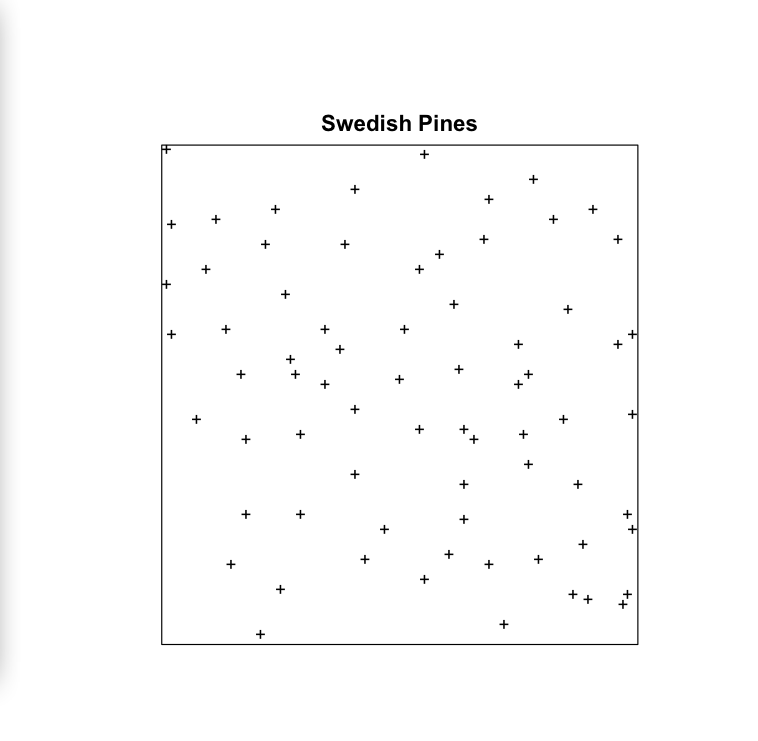
\includegraphics[width=.65\linewidth]{swedish_pines.png}
    \end{center}
  \end{frame}

\begin{frame}[<+->] 
    \frametitle{Quadrat Counts}
    \begin{center}
      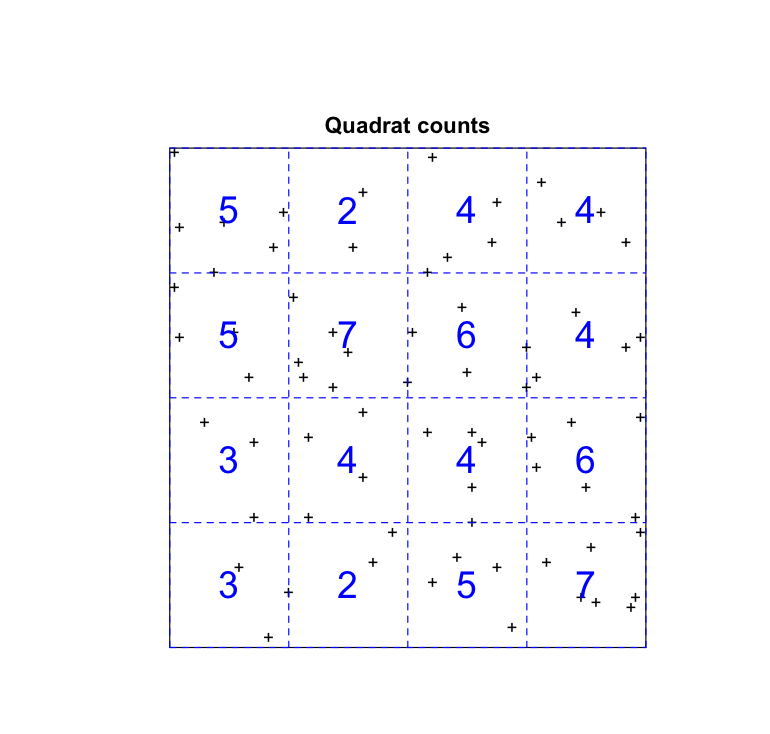
\includegraphics[width=.65\linewidth]{quadrat_counts.png}
    \end{center}
  \end{frame}


\begin{frame}[<+->] 
    \frametitle{Quadrat Counts}
    \begin{center}
      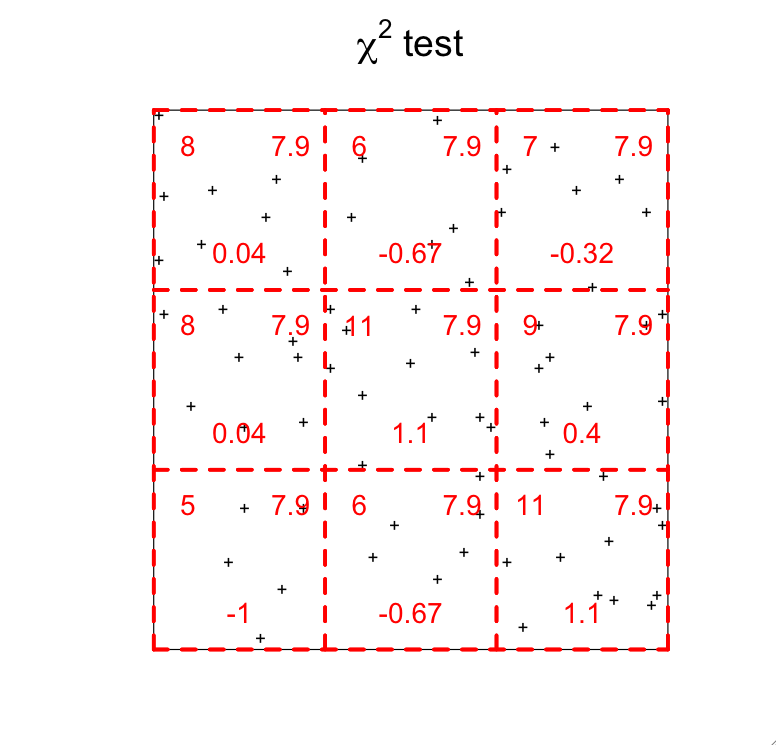
\includegraphics[width=.55\linewidth]{chi_square.png}
    \end{center}
    $\chi^2=4.6761, \ df=8, \ p-value = 0.7916$
  \end{frame}

\begin{frame}[<+->]
  \frametitle{Quadrat Counts}
  \begin{block}{Issues}
    \begin{itemize}
      \item Choice of tessellation
        \begin{itemize}
          \item how many cells?
          \item what cell shape?
          \item locations random or fixed?
        \end{itemize}
      \item Edge effects
      \item Spatial dependence
        \begin{itemize}
          \item Independent cell counts
          \item Independent locations
        \end{itemize}
    \end{itemize}
   \end{block}
 \end{frame}


\begin{frame}[<+->]
  \frametitle{Monte Carlo Simulation}
  \begin{block}{Basic Approach}
    \begin{itemize}
      \item Specify test statistic
      \item Calculate test statistic on observed pattern: $\psi$
      \item Specify a null hypothesis ($H_o$)
      \item Specify an alternate hypothesis ($H_1$)
      \item Simulate Empirical Sampling Distribution of $\psi|H_o$
	\begin{itemize}
	  \item Draw $nsim$ realizations under the null.
	  \item Calculate $\psi_i$ where $i=1,2,\ldots,nsim$.
	  \item Compare $\psi$ to distribution of $\psi_i$.
	\end{itemize}
    \end{itemize}
   \end{block}
 \end{frame}


\subsection{Monte Carlo Simulation}
\begin{frame}[<+->]
  \frametitle{Computational Approximation to Inference}
  \begin{block}{Motivations}
    \begin{itemize}
      \item Substitute capital for labor
      \item Practical when no analytical results are available
      \item Very flexible
    \end{itemize}
   \end{block}
   \begin{block}{Issues}
    \begin{itemize}
      \item Not generalizable beyond data at hand
      \item Less powerful than exact tests (if available)
      \item May be computationally expensive
    \end{itemize}
   \end{block}

 \end{frame}
\begin{frame}[<+->]
  \frametitle{Monte Carlo Simulation}
  \begin{block}{Basic Approach}
    \begin{itemize}
      \item Specify test statistic
      \item Calculate test statistic on observed pattern: $\psi$
      \item Specify a null hypothesis ($H_o$)
      \item Specify an alternate hypothesis ($H_1$)
      \item Simulate Empirical Sampling Distribution of $\psi|H_o$
	\begin{itemize}
	  \item Draw $nsim$ realizations under the null.
	  \item Calculate $\psi_i$ where $i=1,2,\ldots,nsim$.
	  \item Compare $\psi$ to distribution of $\psi_i$.
	\end{itemize}
    \end{itemize}
   \end{block}
 \end{frame}
\subsection{Quadrat Test Example}

  \begin{frame}[containsverbatim]
    \frametitle{Code: ihhpsim.r}
    \begin{small}
      \begin{verbatim}
source("quadcounts.r")
source("ihppsim.r")
pp=ippsim(100)*9+1
ppt=quadcount(pp[,1],pp[,2])
set.seed(100)
nsim=99
source("hppsim.r")
results=matrix(0,nsim+1,1)
for(i in 1:nsim){
    pp=csr(100,1,1,10,10)
    t=quadcount(pp$x,pp$y)
    results[i]=t$chi2
}
results[100]=ppt$chi2
plot(density(results),main="Quadrat Test of Inhomogenous Poisson
Point Process",xlab="Chi^2",ylab="f(Chi^2)")
abline(v=ppt$chi2,col='red')
      \end{verbatim}
    \end{small}
   \end{frame}



\begin{frame}[<+->] 
    \frametitle{Empirical Sampling Distribution}
    \begin{center}
      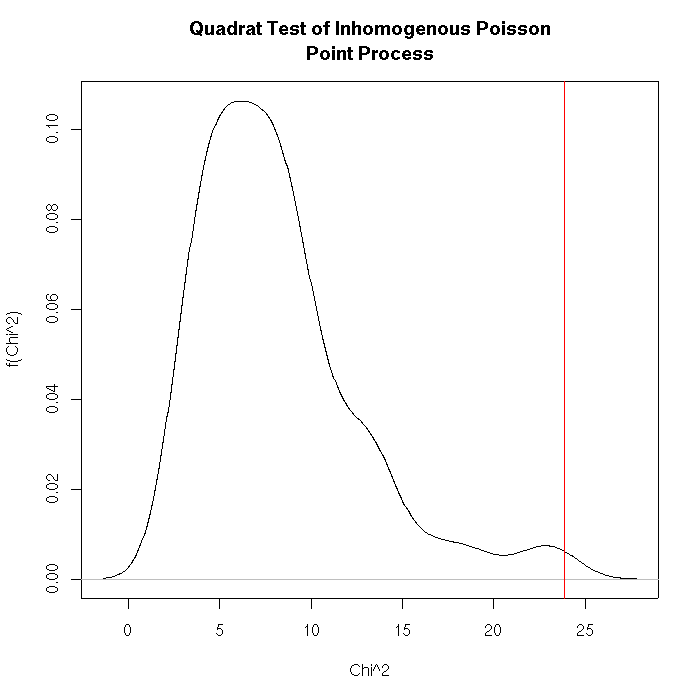
\includegraphics[width=.65\linewidth]{mcsim.png}
    \end{center}
  \end{frame}

\begin{frame}[<+->]
    \frametitle{Pseudo Significance Level}
    \begin{block}{p-value}
      \begin{equation}
	p(\chi^2) = \frac{1+ \sum_{i=1}^{nsim} \psi_i}{nsim+1}
      \end{equation}
      where:
      \begin{equation}
	\psi_{i} = \left\{ \begin{array}{ll}
	  1& if \ \chi_i^2 \ge \chi^2, \\
	  0&otherwise\\
	\end{array} \right.
      \end{equation}
     \end{block}
\begin{block}{p-value}
      \begin{equation}
	\hat{p(\chi^2)} = \frac{1+ 0}{99+1} = 0.01
      \end{equation}
     \end{block}
  \end{frame}


\section{Nearest Neighbor Distance Methods}
\subsection{Mean Nearest Neighbor Statistic}
\begin{frame}[<+->]
  \frametitle{Mean Nearest Neighbor Statistic}
  \begin{block}{$d_{min}(s_i)$}
    \begin{equation}
      d_{min}(s_i) = min(d_{i,1},d_{i,2},\ldots,d_{i,n})
    \end{equation}
   $d_{min}(s_i)$ is the distance between $i$ and its nearest neighbor event.
   \end{block}
  \begin{block}{Test Statistic}
    \begin{equation}
	\bar{d}_{min}= \frac{1}{n} \sum_{i=1}^n d_{min}(s_i)
    \end{equation}
    Originally suggested by Clark and Evans (1954)
   \end{block}
 \end{frame}
\begin{frame}[<+->]
  \frametitle{Mean Nearest Neighbor Statistic Distribution}
  \begin{block}{$\bar{d}_{min}^{\sim}N(\mu,\sigma^2)$}
    \begin{equation}
      \mu=E[\bar{d}_{min}] = 0.5(n^{-1} |A|)^{1/2} + (0.051 + 0.042n^{-1/2})n^{-1}
      P
    \end{equation}
    \begin{equation}
      \sigma^2 = V[\bar{d}_{min}] =0.070n^{-1/2} |A| + 0.037(n^{-5}|A|)^{1/2}P
    \end{equation}
    where $|A|$ and $P$ are the area and perimeter of the study area,
    respectively.
   \end{block}
   \begin{block}{Issues}
     \begin{itemize}
       \item Approximation, not an exact result.
       \item Dependence of nearest neighbor distances is ignored.
       \item Distribution of $d_{min}(s_i)$ ignored (only first moment).
     \end{itemize}
   \end{block}
 \end{frame}



  \begin{frame}[<+->]
    \frametitle{Edge Effects}
    \begin{block}{Problems}
      \begin{itemize}
	\item For points close the the boundary intensity is underestimated.
	\item Neighboring points are outside the study region.
      \end{itemize}
\end{block}
      \begin{block}{Solutions}
	\begin{itemize}
	  \item Buffer the points
	  \item Edge corrections
	  \item Monte Carlo Simulations
	\end{itemize}
      \end{block}
   \end{frame}

\subsection{Nearest Event-Event Neighbor Distance Functions}

\begin{frame}[<+->]
    \frametitle{Nearest Neighbor G Function}
    \begin{block}{$G(d)$}
      \begin{equation}
	G(d) = \sum_{i=1}^n \Phi_{i}^d / n
      \end{equation}
      where
\begin{equation}
	\Phi_{i}^d = \left\{ \begin{array}{ll}
	  1& if \ d_{min}(s_i) < d \\
	  0&otherwise\\
	\end{array} \right.
      \end{equation}
      $G(d)$ is the proportion of nearest neighbor distances that are less
      than $d$.
    \end{block}
  \end{frame}

\begin{frame}[<+->]
    \frametitle{Uganda Crater Data}
    \begin{center}
      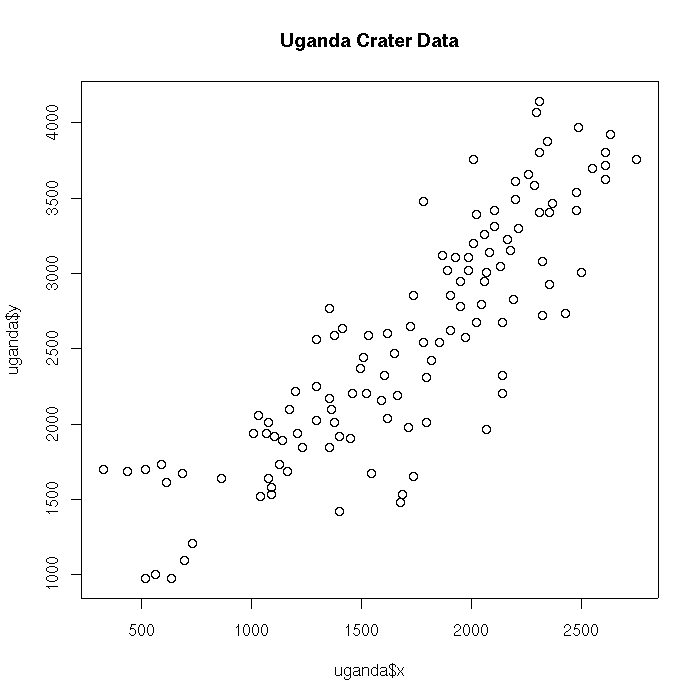
\includegraphics[width=.65\linewidth]{uganda.png}
    \end{center}
  \end{frame}


\begin{frame}[<+->]
    \frametitle{Nearest Neighbor G Function}
    \begin{center}
      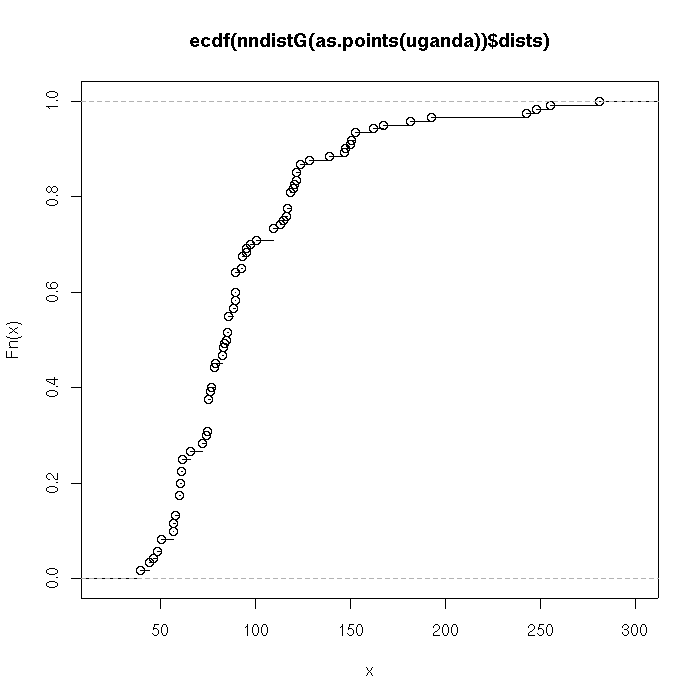
\includegraphics[width=.65\linewidth]{nng.png}
    \end{center}
  \end{frame}
  \begin{frame}[<+->]

    \frametitle{G Function Intepretation}
    \begin{block}{Shape}
      \begin{itemize}
	\item G increasing rapidly at small distances points to
	  \emph{clustering}.
	\item G increases slowly points to \emph{uniformity}.
	\item Both are deviations from CSR.
      \end{itemize}
     \end{block}
\begin{block}{Compare G to that from a CSR Process}
      \begin{itemize}
	\item Theoretical G
	    \item Homogeneous Poisson process
	    \item Density equal to density of actual pattern
	\item Empirical distribution against theoretical distribution
	  \begin{itemize}
	    \item Should be a 45 degree line if process is CSR
	    \item Above the line = clustering
	    \item Below the line = dispersion
	  \end{itemize}
      \end{itemize}
     \end{block}


   \end{frame}


\begin{frame}[<+->]
    \frametitle{Nearest Neighbor G Function}
    \begin{center}
      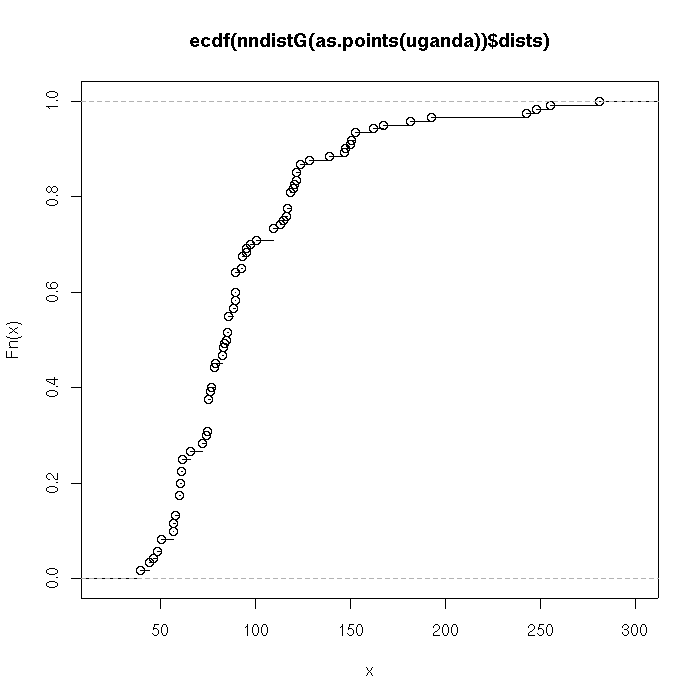
\includegraphics[width=.65\linewidth]{nng.png}
    \end{center}
  \end{frame}


  \begin{frame}[containsverbatim]
    \frametitle{Estimated vs. Theoretical G Function: Code}
    \begin{small}
      \begin{verbatim}
> library(splancs)
> data(uganda)
> plot(Ghat(as.points(uganda), seq(20, 500, 20)),
+ Fzero(pdense(as.points(uganda),  uganda$poly),
+ seq(20, 500, 20)), type="l", 
+ xlab="Theoretical G", 
+ ylab="Estimated G")
> lines(c(0,1),c(0,1),lty=2)
      \end{verbatim}
    \end{small}
   \end{frame}


\begin{frame}[<+->]
    \frametitle{Estimated vs. Theoretical G Function}
    \begin{center}
      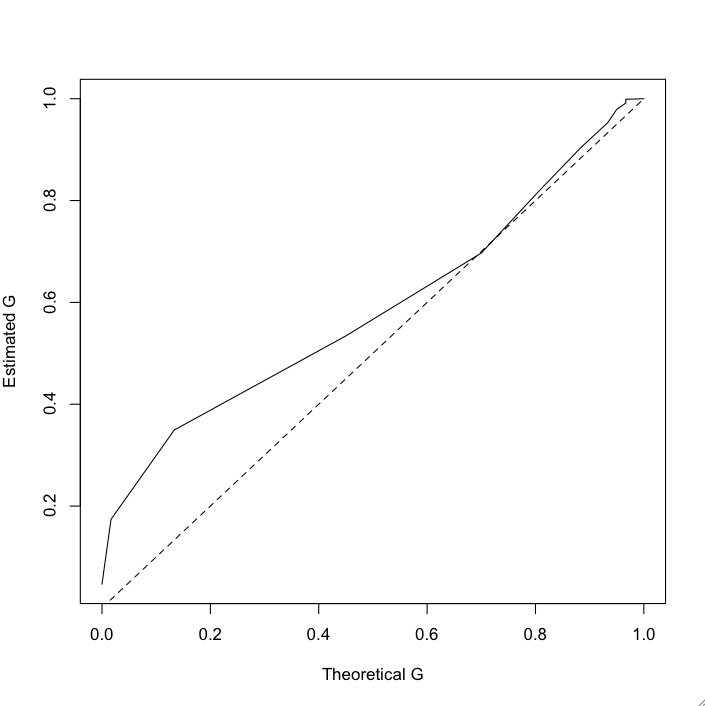
\includegraphics[width=.65\linewidth]{theoryg.png}
    \end{center}
  \end{frame}


\subsection{Nearest Point-Event Neighbor Distances}

\begin{frame}[<+->]
    \frametitle{Nearest Neighbor F Function}
    \begin{itemize}
      \item G function is sensitive to $n$
	\begin{itemize}
	  \item Can be rough
	  \item Takes on stepped appearance for small $n$
	\end{itemize}
      \item Alternative approach is to generate $N$ random points in the
	domain
	\begin{itemize}
	  \item Analyze the distribution of nearest event neighbor distances
	  \item Closest event to each point.
	\end{itemize}
      \item Can be used for small $n$ data sets
    \end{itemize}
  \end{frame}


\begin{frame}[<+->]
    \frametitle{Nearest Neighbor F Function}
    \begin{center}
      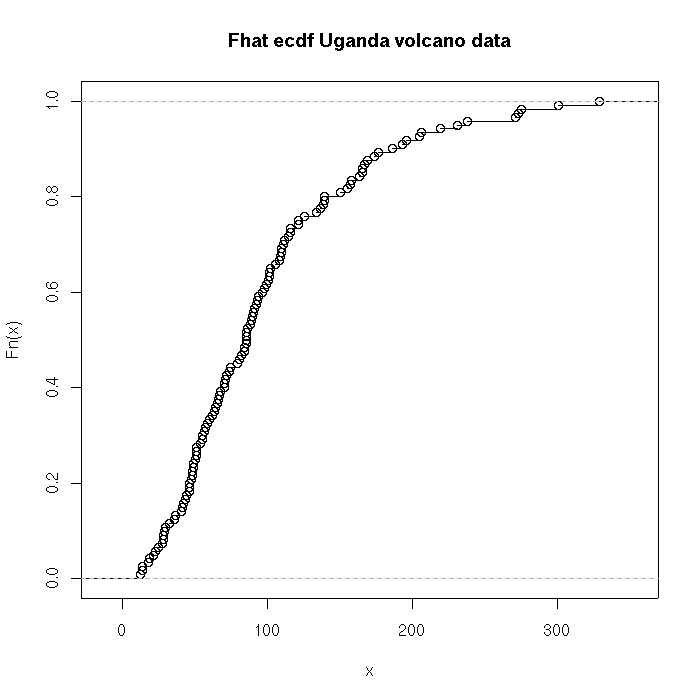
\includegraphics[width=.65\linewidth]{nnf.png}
    \end{center}
  \end{frame}

\begin{frame}[<+->]
    \frametitle{Nearest Neighbor J Function}
    \begin{equation}
      J(d) = (1-G(d))/(1-F(d))
      \label{e:j}
    \end{equation}
    \begin{itemize}
      \item $J(d) < 1$ points to spatial clustering
      \item $J(d) > 1$ points to spatial regularity
    \end{itemize}
  \end{frame}

\begin{frame}[<+->]
    \frametitle{Redwood}
    \begin{center}
      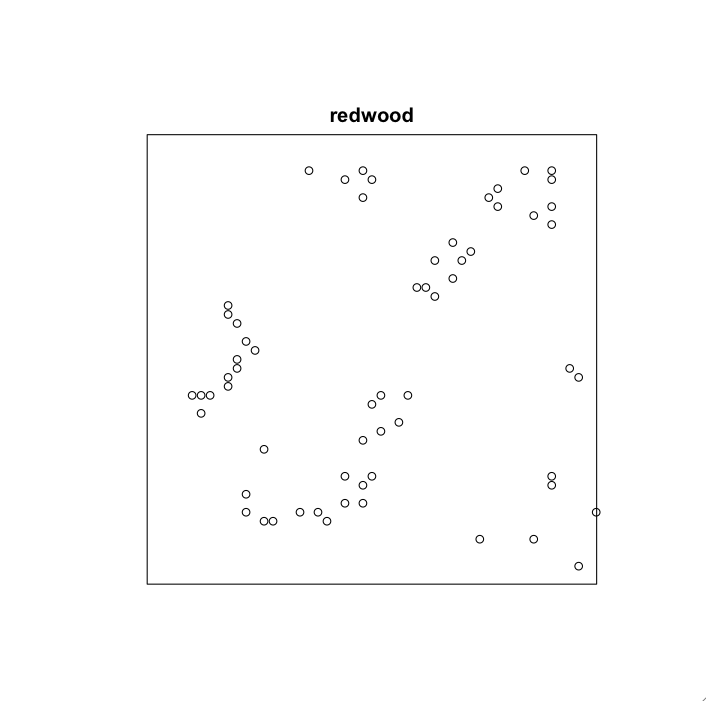
\includegraphics[width=.65\linewidth]{redwood.png}
    \end{center}
  \end{frame}

  \begin{frame}[containsverbatim]
    \frametitle{R code}
    \begin{small}
      \begin{verbatim}
> gr=Gest(redwood)
> plot(gr,main="G for Redwood")
     lty col
km     1   1
rs     2   2
theo   3   3
      \end{verbatim}
      \begin{itemize}
	\item $km$: spatial Kaplan-Meier estimator of $G(r)$
	\item $rs$: the reduced sample edge correction estimator of $G(r)$
	\item $theo$: the theoretical value of $G(r)$ for a CSR process
      \end{itemize}
    \end{small}
   \end{frame}


\begin{frame}[<+->]
    \frametitle{Nearest Neighbor G Function}
    \begin{center}
      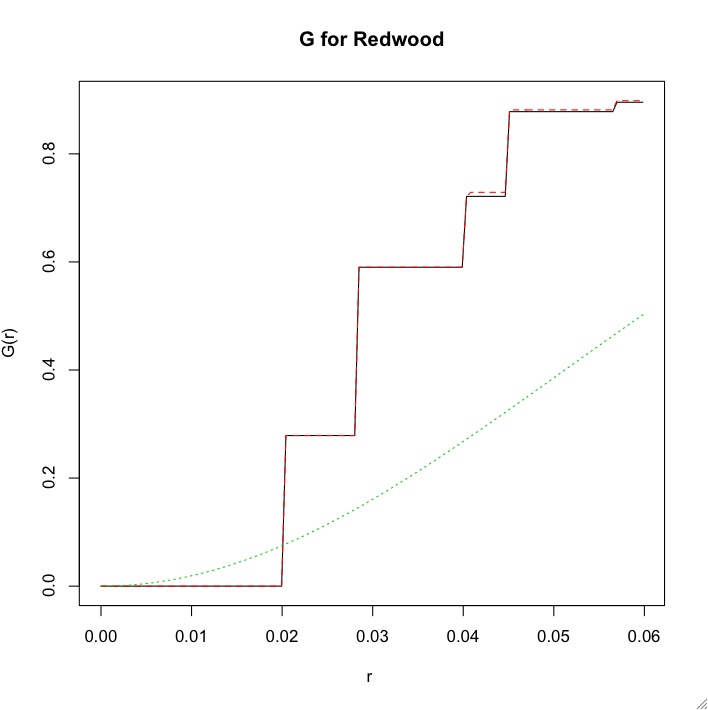
\includegraphics[width=.65\linewidth]{gredwood.png}
    \end{center}
  \end{frame}

\begin{frame}[<+->]
    \frametitle{Nearest Neighbor F Function}
    \begin{center}
      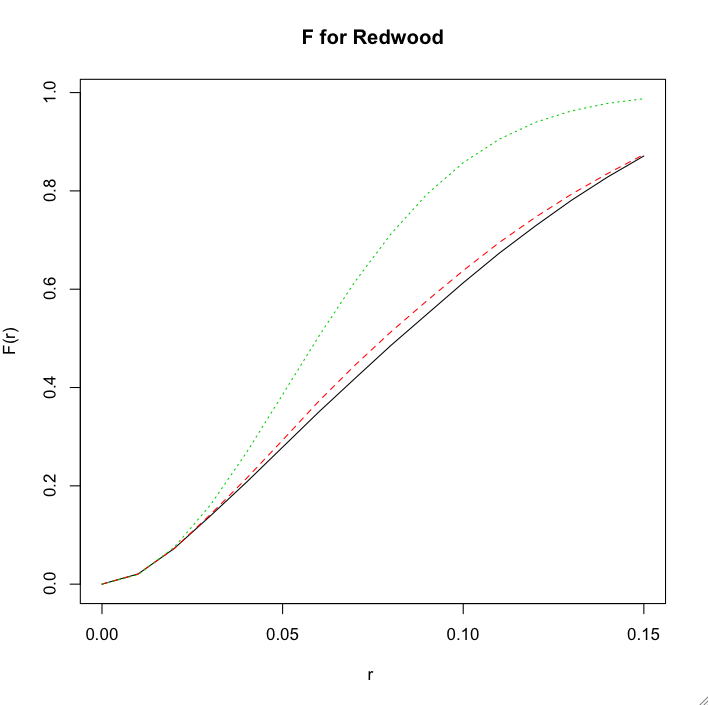
\includegraphics[width=.65\linewidth]{fredwood.png}
    \end{center}
  \end{frame}

  \begin{frame}[containsverbatim]
    \frametitle{R code: J Function}
    \begin{small}
      \begin{verbatim}

>    J <- Jest(redwood, 0.01)
>    plot(J, main="redwood data")
     lty col
km     1   1
rs     2   2
un     3   3
theo   4   4
>    # values are below J= 1, indicating clustered pattern
      \end{verbatim}
      \begin{itemize}
	\item $km$: spatial Kaplan-Meier estimator of $G(r)$
	\item $rs$: the reduced sample edge correction estimator of $G(r)$
	\item $un$: the uncorrected estimate of $J(r)$ computed from the
	  uncorrected estimates of $F$ and $G$
	\item $theo$: the theoretical value of $J(r)$ for a CSR process
      \end{itemize}
    \end{small}
   \end{frame}



\begin{frame}[<+->]
    \frametitle{Nearest Neighbor J Function}
    \begin{center}
      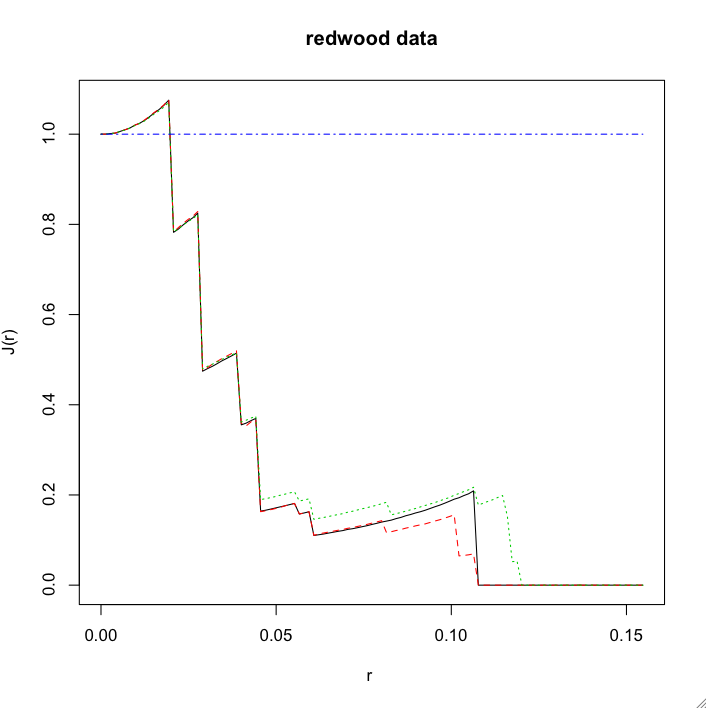
\includegraphics[width=.65\linewidth]{jredwood.png}
    \end{center}
  \end{frame}

 \section{Inter-Event Distance Distributions}
 \begin{frame}[<+->]
   \frametitle{Inter-Event Distance Distributions}
   \begin{block}{$G$, $F$, and $J$ Functions}
     \begin{itemize}
       \item Take account of the nearest neighbor distributions: $n$ distances
	 or pieces of
	 information
       \item Do not account for the full distribution of inter-event distances
	 $n(n-1)/2$ distances.
     \end{itemize}
\end{block}
     \begin{block}{Inter-Event Distances}
       \begin{itemize}
	 \item Consider all inter-event distances
	 \item More than one distance for each point
	 \item Second order analysis
	   \begin{itemize}
	     \item Expresses the dependence of events
	     \item Spatial interaction
	   \end{itemize}
       \end{itemize}
     \end{block}
  \end{frame}

  \begin{frame}[<+->]
    \frametitle{Ripley's $K$ function}
    \begin{block}{$K$}
      \begin{equation}
	K(d) = \frac{\sum_{i=1}^n \sum_{j=1}^n \psi_{ij}(d)}{n\lambda}
      \end{equation}
where:
      \begin{equation}
	\psi_{ij}(d) = \left\{ \begin{array}{ll}
	  1& if \ d_{ij} \le d \\
	  0&otherwise\\
	\end{array} \right.
      \end{equation}

     \end{block}
     \begin{block}{Circle centered on each point $s_i$}
       \begin{equation}
	 \sum_{j=1}^n \psi_{ij}(d)
       \end{equation}
       is the number of events within a circle of radius $d$ centered on even
       $s_i$.
     \end{block}
   \end{frame}

  \begin{frame}[containsverbatim]
    \frametitle{R code: K Function}
    \begin{small}
      \begin{verbatim}
> rk=Kest(redwood)
> plot(rk,main="K function for redwood")
       lty col
iso      1   1
trans    2   2
border   3   3
theo     4   4
      \end{verbatim}
      \begin{itemize}
	\item $iso$: Ripley's isotropic correction.
	\item $trans$: Translation correction.
	\item $border$: reduced sample estimator.
	\item $theo$: the theoretical value of $K$
      \end{itemize}
    \end{small}
   \end{frame}

\begin{frame}[<+->]
    \frametitle{K function}
    \begin{center}
      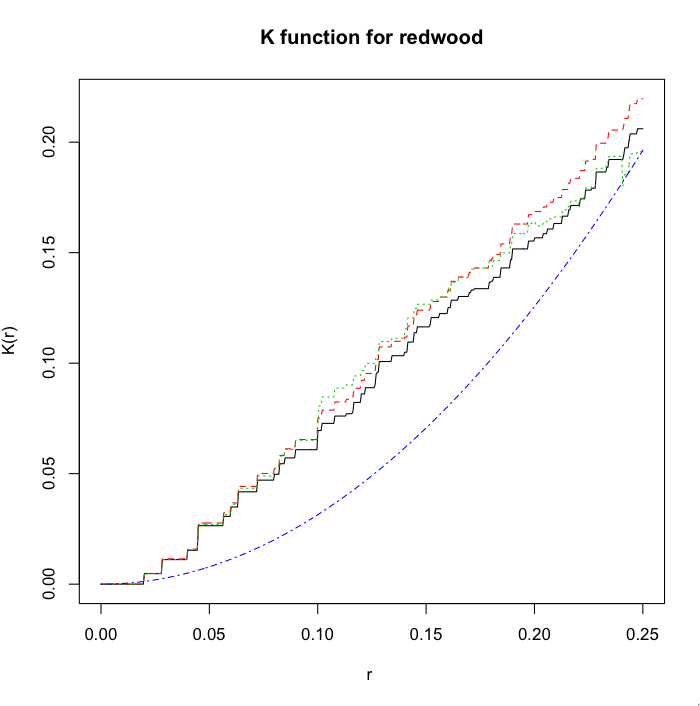
\includegraphics[width=.65\linewidth]{kredwood.png}
    \end{center}
  \end{frame}
 
\begin{frame}[<+->]
    \frametitle{$L$ function}
    \begin{block}{Scaling of $K$}
      \begin{equation}
	L(d) = \sqrt{ K(d)/\pi } - d
      \end{equation}
    \end{block}
    \begin{block}{ Useful since:}
    \begin{equation}
      E[K(d)] = \frac{\pi \lambda d^2}{\lambda}
    \end{equation}
    which can get large with $d^2$ and obscures small differences between
    expected and observed values.
  \end{block}
  \end{frame}
 

  \begin{frame}[containsverbatim]
    \frametitle{R code: L Function}
    \begin{small}
      \begin{verbatim}

>  plot(rk, sqrt(./pi) ~ r, ylab="L(r)", 
    + main="L function for redwood")
       lty col
iso      1   1
trans    2   2
border   3   3
theo     4   4
> 
      \end{verbatim}
      \begin{itemize}
	\item $iso$: Ripley's isotropic correction.
	\item $trans$: Translation correction.
	\item $border$: reduced sample estimator.
	\item $theo$: the theoretical value of $K$
      \end{itemize}
    \end{small}
   \end{frame}

\begin{frame}[<+->]
    \frametitle{L function}
    \begin{center}
      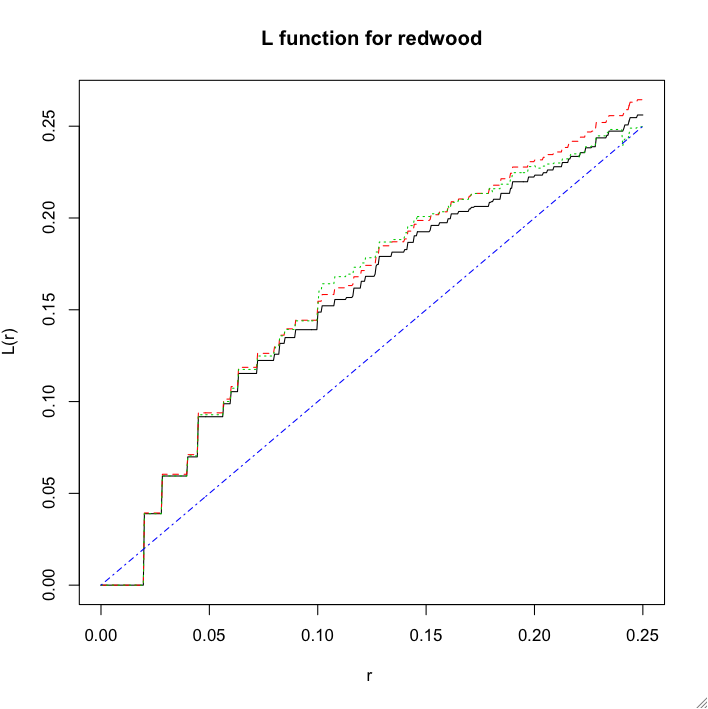
\includegraphics[width=.65\linewidth]{lredwood.png}
    \end{center}
  \end{frame}
 





  \begin{frame}[containsverbatim]
    \frametitle{Simulation envelopes for $K$}
    \begin{small}
      \begin{verbatim}
> plot(envelope(redwood))
Generating 99 simulations of CSR ...
1, 2, 3, 4, 5, 6, 7, 8, 9, 10, 11, 12, 13, 14, 15,
16, 17, 18, 19, 20, 21, 22, 23, 24, 25, 26, 27, 28, 29, 30,
31, 32, 33, 34, 35, 36, 37, 38, 39, 40, 41, 42, 43, 44, 45,
46, 47, 48, 49, 50, 51, 52, 53, 54, 55, 56, 57, 58, 59, 60,
61, 62, 63, 64, 65, 66, 67, 68, 69, 70, 71, 72, 73, 74, 75,
76, 77, 78, 79, 80, 81, 82, 83, 84, 85, 86, 87, 88, 89, 90,
91, 92, 93, 94, 95, 96, 97, 98, 99.

Done.
     lty col
obs    1   1
theo   2   2
hi     3   3
lo     4   4

      \end{verbatim}
    \end{small}
   \end{frame}



\begin{frame}[<+->]
    \frametitle{K function simulation}
    \begin{center}
      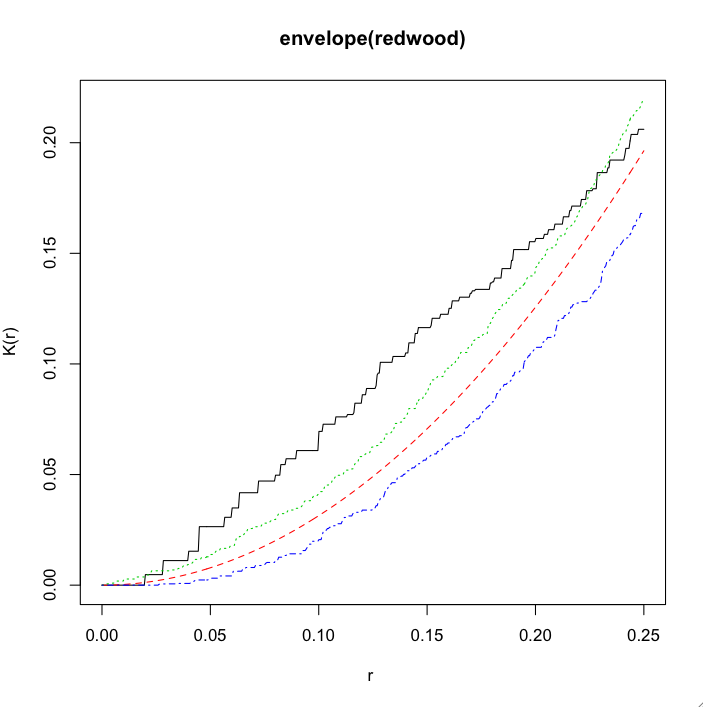
\includegraphics[width=.65\linewidth]{ksimredwood.png}
    \end{center}
  \end{frame}

  \begin{frame}[containsverbatim]
    \frametitle{Simulation envelopes for $L$}
    \begin{small}
      \begin{verbatim}
> E=envelope(redwood,Kest)
Generating 99 simulations of CSR ...
1, 2, 3, 4, 5, 6, 7, 8, 9, 10, 11, 12, 13, 14, 15,
16, 17, 18, 19, 20, 21, 22, 23, 24, 25, 26, 27, 28, 29, 30,
31, 32, 33, 34, 35, 36, 37, 38, 39, 40, 41, 42, 43, 44, 45,
46, 47, 48, 49, 50, 51, 52, 53, 54, 55, 56, 57, 58, 59, 60,
61, 62, 63, 64, 65, 66, 67, 68, 69, 70, 71, 72, 73, 74, 75,
76, 77, 78, 79, 80, 81, 82, 83, 84, 85, 86, 87, 88, 89, 90,
91, 92, 93, 94, 95, 96, 97, 98, 99.

Done.
> plot(E,sqrt(./pi)~r,main="L simulation envelopes")
     lty col
obs    1   1
theo   2   2
hi     3   3
lo     4   4
      \end{verbatim}
    \end{small}
   \end{frame}


\begin{frame}[<+->]
    \frametitle{L function simulation}
    \begin{center}
      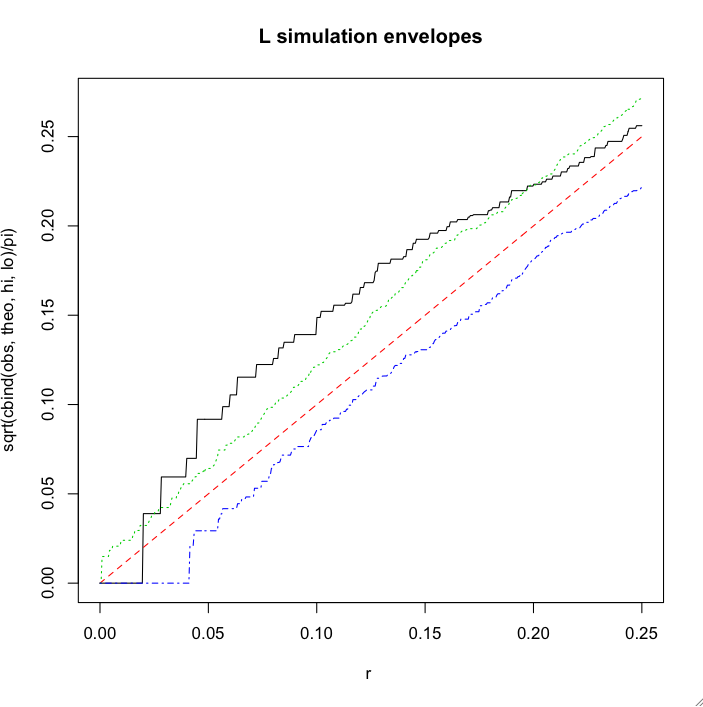
\includegraphics[width=.65\linewidth]{lsimredwood.png}
    \end{center}
  \end{frame}

\begin{frame}[<+->]
    \frametitle{G function simulation}
    \begin{center}
      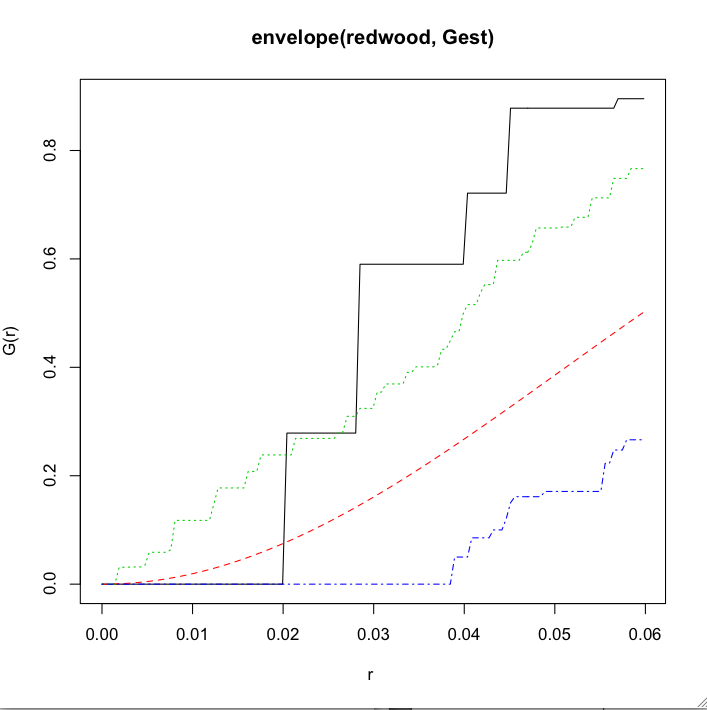
\includegraphics[width=.65\linewidth]{gsimredwood.png}
    \end{center}
  \end{frame}


\begin{frame}[<+->]
    \frametitle{F function simulation}
    \begin{center}
      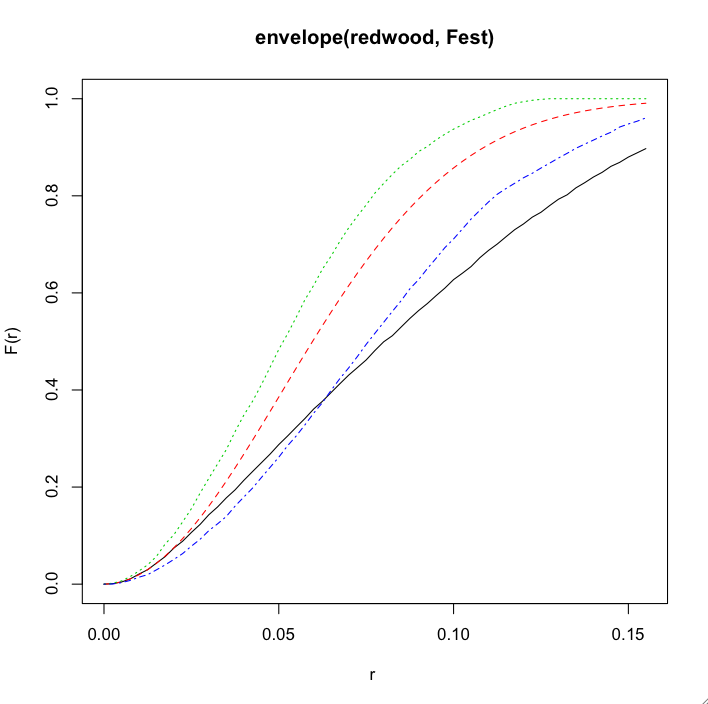
\includegraphics[width=.65\linewidth]{fsimredwood.png}
    \end{center}
  \end{frame}



\end{document}


